\section{Describing Relationships}

\subsection{Scatterplots}

A \textbf{scatterplot} displays the relationship between two quantitative variables measured on the same individuals. Mark values of one variable on the horizontal axis ($x$-axis) and values of the other variable on the vertical axis ($y$-axis). Plot each individual's data as a point on the graph.

\begin{definition}{Scatterplot}{}
    A \textbf{scatterplot} shows the relationship between two quantitative variables measured on the same individuals. The values of one variable appear on the horizontal axis, and the values of the other variable appear on the vertical axis. Each individual in the data appears as a point in the graph.
\end{definition}

If we think that a variable $x$ may help explain, predict, or even cause changes in another variable $y$, we call $x$ an \textbf{explanatory variable} and $y$ a \textbf{response variable}. Always plot the explanatory variable, if there is one, on the $x$ axis of a scatterplot. Plot the response variable on the $y$ axis. If there is no explanatory-response distinction, either variable can go on the horizontal axis.

In examining a scatterplot, look for an overall pattern showing the \textbf{direction}, \textbf{form}, and \textbf{strength} of the relationship and then look for \textbf{outliers} or other departures from this pattern.

\begin{itemize}[font=\sffamily\bfseries, leftmargin=1.95cm, style=nextline, itemsep=0cm]
\item[Direction] If the relationship has a clear direction, we speak of either \textit{positive association} or \textit{negative association}.
\item[Form] \textit{Linear relationships}, where the points show a straight-line pattern, are an important form of relationship between two variables. \textit{Curved relationships} and clusters are other forms to watch for.
\item[Strength] The strength of a relationship is determined by \textit{how close} the points in the scatterplot lie to a simple form such as a line.
\end{itemize}

\subsection{Correlation}

The \textbf{correlation} $r \in [-1, +1]$ measures the \textit{strength} and \textit{direction} of the \textit{linear association} between two quantitative variables $x$ and $y$. Although you can calculate a correlation for \textit{any} scatterplot, $r$ measures strength for \textit{only} straight-line relationships.

Correlation indicates the direction of a linear relationship by its sign and magnitude:

\begin{itemize}[itemsep=0cm]
\item $r > 0$ for a positive association;
\item $r < 0$ for a negative association;
\item $r = \pm 1$ occurs only when the points on a scatterplot lie exactly on a straight line; and
\item $|r|$ indicates the strength of a linear relationship by how close it is to -1 or +1.
\end{itemize}

\begin{definition}{Correlation}{}
    The \textbf{correlation} $r$ measures the direction and strength of the linear relationship between two quantitative variables. \\
    Suppose that we have data on variables $x$ and $y$ for $n$ individuals given as:
    \[
        (x_1, y_1), (x_2, y_2), ..., (x_n, y_n).
    \]
    The means and standard deviations of the two variables are $\bar{x}$ and $s_x$ for the $x$-values, and $\bar{y}$ and $s_y$ for the $y$-values. The correlation $r$ between $x$ and $y$ is given by
    \begin{align*}
        r
        = \dfrac{1}{n-1} \sum_{i=1}^{n}
            \left( \dfrac{x_i - \bar{x}}{s_x} \right)
            \left( \dfrac{y_i - \bar{y}}{s_y} \right)
        = \dfrac{1}{n-1} \sum_{i=1}^{n} z_{x_i} z_{y_i}.
    \end{align*}
\end{definition}

\begin{figure}[ht!]
    \centering
    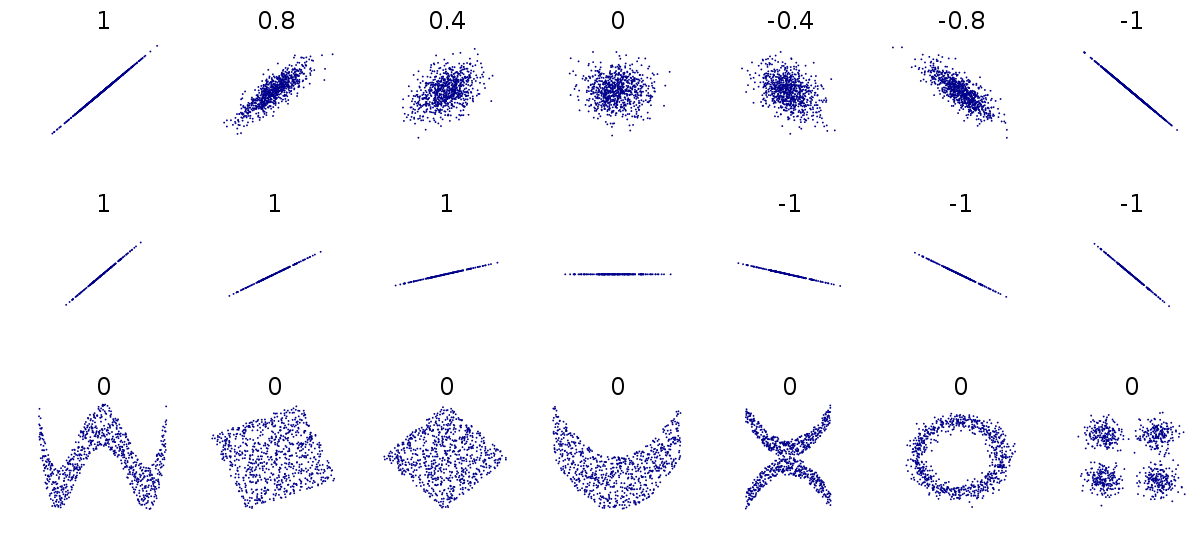
\includegraphics[width=\linewidth]{ch03/correlation.png}
    \caption{Several sets of $(x, y)$ points, with the correlation coefficient of $x$ and $y$ for each set. The correlation reflects the noisiness and direction of a linear relationship (top row), but not the slope of that relationship (middle), nor many aspects of nonlinear relationships (bottom). N.B.: the figure in the center has a slope of 0 but in that case the correlation coefficient is undefined because the variance of $y$'s is zero.}
\end{figure}

How correlation behaves is more important than the details of the formula. Here's what you need to know in order to interpret correlation correctly.

\begin{itemize}[itemsep=0cm]
\item Correlation makes no distinction between explanatory and response variables.
\item Because $r$ uses the standardized values of the observations, $r$ does not change when we change the units of measurement of $x$, $y$, or both.
\item The correlation $r$ itself has no unit of measurement.
\end{itemize}

Describing the relationship between two variables is more complex than describing the distribution of one variable. Here are some cautions to keep in mind when you use correlation.

\begin{itemize}[itemsep=0cm]
\item Correlation does not imply causation.
\item Correlation requires that both variables be quantitative, so that it makes sense to do the arithmetic indicated by the formula for $r$.
\item Correlation only measures the strength of a \textit{linear relationship} between two variables, i.e., it does not describe \textit{curved relationships} between variables, no matter how strong the relationship is.
\item A value of $r$ close to $1$ or $-1$ does not guarantee a linear relationship between two variables, e.g., when the underlying relationship is curved but not linear.
\item Like mean and standard deviation, the correlation is not resistant: $r$ is strongly affected by a few outlying observations. Use $r$ with caution when outliers appear in the scatterplot.
\item Correlation is not a complete summary of two-variable data, even when the relationship between the variables is linear. You should give the means and standard deviations of both $x$ and $y$ along with the correlation.
\end{itemize}

\subsection{Linear Regression}

A \textbf{regression} line is a \textit{model} for the data. It summarizes the relationship between two variables, but only in a specific setting: when one of the variables helps explain or predict the other. Regression, unlike correlation, requires that we have an explanatory variable and a response variable.

\begin{definition}{Regression line}{}
    A \textbf{regression line} is a line that describes how a response variable $y$ changes as an explanatory variable $x$ changes. We often use a regression line to predict the value of $y$ for a given value of $x$. \\
    Suppose that $y$ is a response variable (plotted on the vertical axis) and $x$ is an explanatory variable (plotted on the horizontal axis). A regression line relating $y$ to $x$ has an equation of the form
    \[
        \hat{y} = a + bx,
    \]
    where
    \begin{itemize}[itemsep=0cm]
    \item $\hat{y}$ (read ``$y$ hat'') is the \textbf{predicted value} of the response variable $y$ for a given value of the explanatory variable $x$;
    \item $b$ is the \textbf{slope}, the amount by which $y$ is predicted to change when $x$ increases by one unit; and
    \item $a$ is the \textbf{$\mathbf{y}$-intercept} the predicted value of $y$ when $x = 0$.
    \end{itemize}
\end{definition}
Few relationships are linear for \textit{all} values of the explanatory variable. Don't make predictions using values of $x$ that are \textit{much larger} or \textit{much smaller} than those that actually appear in your data.

A good regression line makes the vertical deviations of the points from the line as small as possible. These vertical deviations represent ``leftover'' variation in the response variable after fitting the regression line. For that reason, they are called \textbf{residuals}.

\begin{definition}{Residual}{}
    A \textbf{residual} is the difference between an observed value of the response variable and the value predicted by the regression line, i.e.,
    \begin{align*}
        \text{residual}
        &= \text{observed $y$} - \text{predicted $y$} \\
        &= y - \hat{y}.
    \end{align*}
\end{definition}

The regression line we want is the one that minimizes the sum of the squared residuals.

\begin{definition}{Least-squares regression line}{}
    The \textbf{least-squares regression line} of $y$ on $x$ is the line that makes the sum of the squared residuals as small as possible.\\
    Suppose that we have data on variables $x$ and $y$ for $n$ individuals given as:
    \[
        (x_1, y_1), (x_2, y_2), ..., (x_n, y_n).
    \]
    The means and standard deviations of the two variables are $\bar{x}$ and $s_x$ for the $x$-values, and $\bar{y}$ and $s_y$ for the $y$-values. The least-squares regression line is the line $\hat{y} = a + bx$ where
    \[
        b = r \dfrac{s_y}{s_x} \quad\text{and}\quad
        a = \bar{y} - b \bar{x}.
    \]
\end{definition}

Note that when displaying the equation of a least-squares regression line, the calculator will report the slope and intercept with much more precision than we need. However, there is no firm rule for how many decimal places to show for answers on the AP exam. The advice is that decide how much to round based on the context of the problem you are working on.

Although residuals can be calculated from any model that is fitted to the data, the residuals from the least-squares line have a special property: the mean of the least-squares residuals is \textit{always} zero.

Correlation and regression are powerful tools for describing the relationship between two variables. When you use these tools, you should be aware of their limitations.

\begin{itemize}[itemsep=0cm]
\item The distinction between explanatory and response variables is important in regression.
\item Correlation and regression lines describe only linear relationships, i.e., the results are useful only if the scatterplot shows a linear pattern. Always plot your data. See also Figure \ref{fig:anscombe}.
\item Correlation and least-squares regression lines are not resistant. One unusual point in a scatterplot can greatly change the value of $r$. Least-squares lines make the sum of the squares of the vertical distances to the points as small as possible. A point that is extreme in the $x$ direction with no other points near it pulls the line toward itself. We call such points \textbf{influential}. See also Figure \ref{fig:anscombe} and \ref{fig:regression-outlier}.
\item Association does not imply causation. A strong association between two variables is not enough to draw conclusions about cause and effect.
\end{itemize}

\begin{definition}{Outliers and influential observations in regression}{}
    An \textbf{outlier} is an observation that lies outside the overall pattern of the other observations. Points that are outliers in the $y$ direction but not the $x$ direction of a scatterplot have large residuals. Other outliers may not have large residuals. \\
    An observation is \textbf{influential} for a statistical calculation if removing it would markedly change the result of the calculation. Points that are outliers in the $x$ direction of a scatterplot are often influential for the least-squares regression line.
\end{definition}

\begin{figure}[ht!]
    \centering
    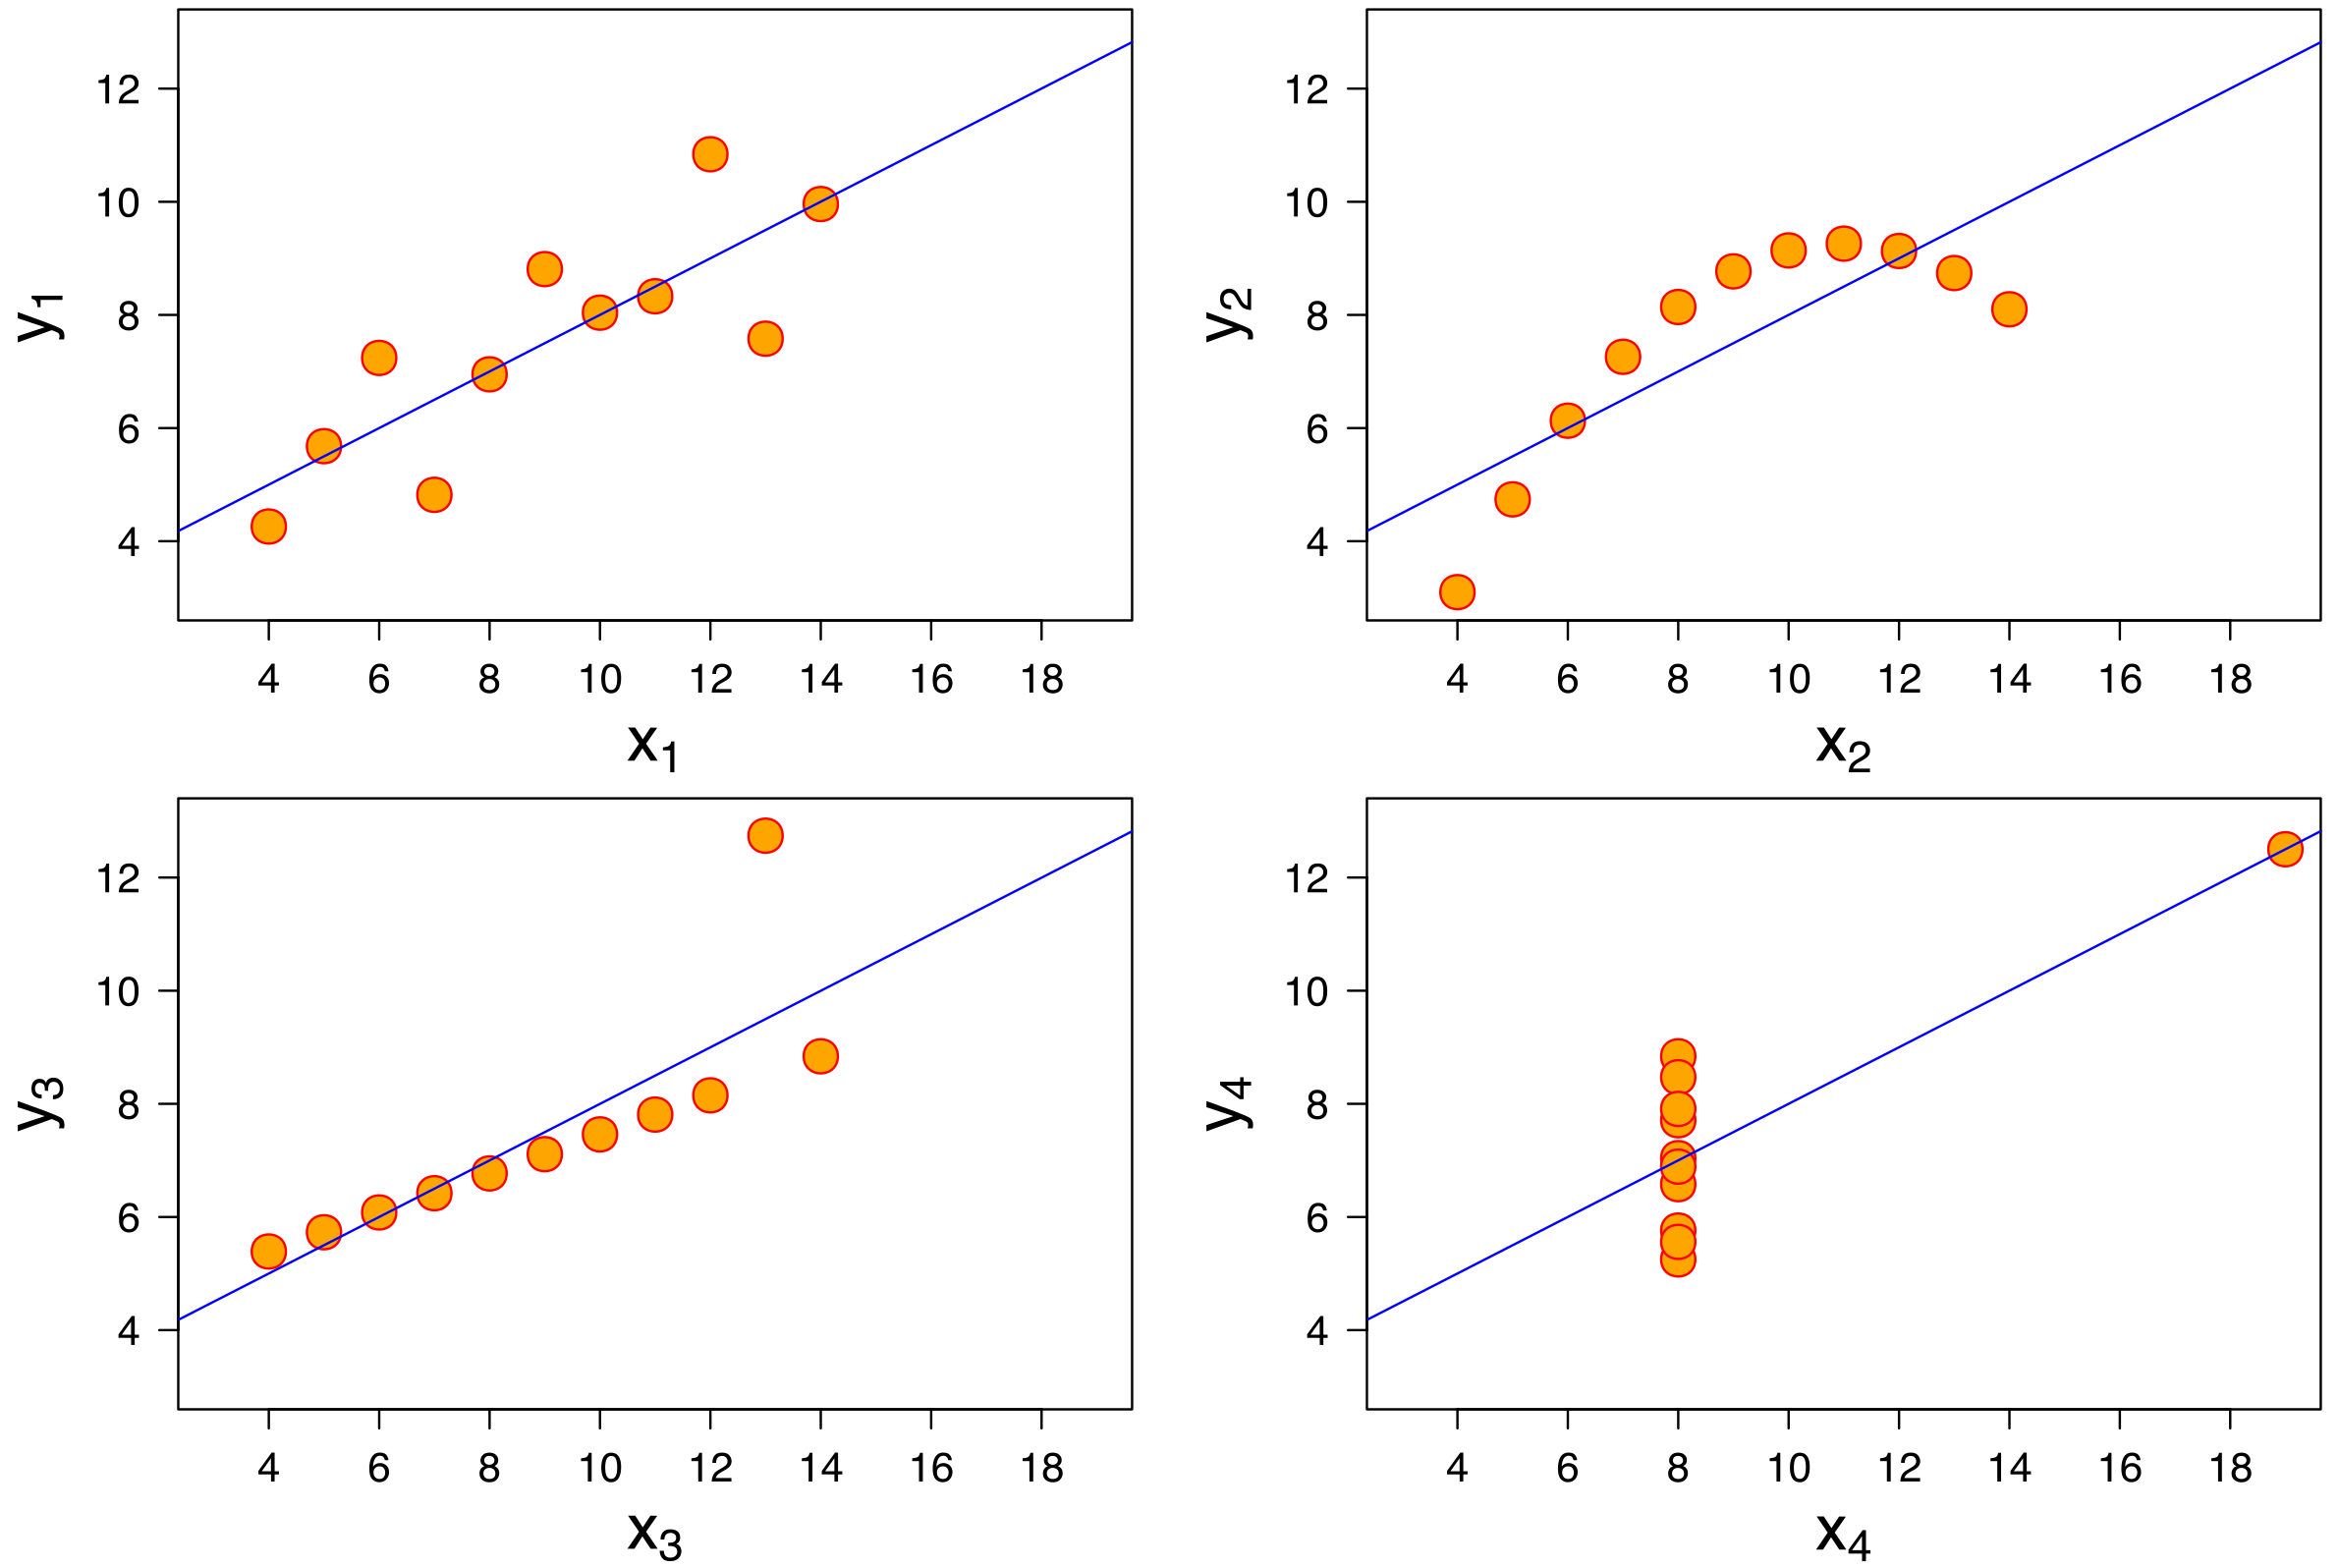
\includegraphics[width=0.9\linewidth]{ch03/anscombe.png}
    \caption{All four sets are identical when examined using simple summary statistics, but vary considerably when graphed. $\bar{x} = 9$, $\bar{y} = 7.50$, $s_x^2 = 11$, $s_y^2 = 4.125$, correlation $r = 0.816$, linear regression line $\hat{y} = 3.00 + 0.500x$, coefficient of determination $r^2 = 0.67$.}
    \label{fig:anscombe}
\end{figure}

\begin{figure}[ht!]
    \centering
    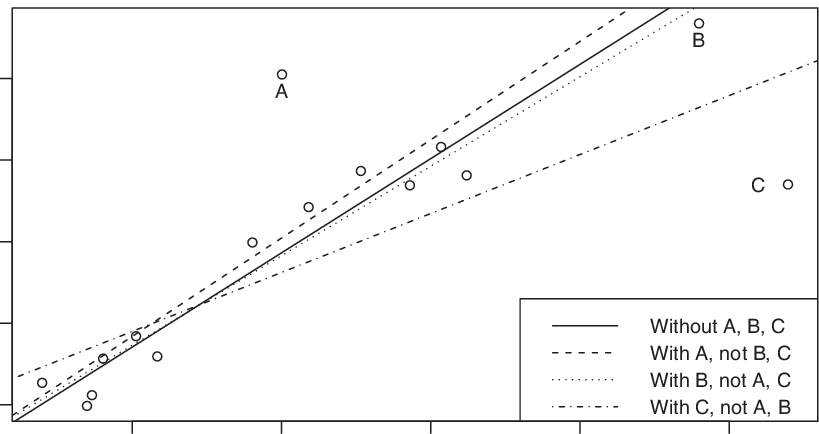
\includegraphics[width=0.6\linewidth]{ch03/regression-outlier.png}
    \caption{Outliers in regression are observations that fall far from the ``cloud'' of points. These points are especially important because they can have a strong influence on the least squares line.}
    \label{fig:regression-outlier}
\end{figure}

\subsubsection{Residual Plot}

A \textbf{residual plot} in effect turns the regression line horizontal. It magnifies the deviations of the points from the line, making it easier to see unusual observations and patterns.

\begin{definition}{Residual plot}{}
    A \textbf{residual plot} is a scatterplot of the residuals against the explanatory variable. Residual plots help us assess whether a linear model is appropriate.
\end{definition}

When an obvious curved pattern exists in a residual plot, the model we are using is not appropriate. Remember when we calculate a residual, we are calculating what is left over after subtracting the predicted value from the observed value:
\[
    \text{residual} = \text{observed $y$} - \text{predicted $y$}.
\]
Likewise, when we look at the form of a residual plot, we are looking at the form that is left over after subtracting the form of the model from the form of the association:
\[
    \text{form of residual plot}
    = \text{form of association}
    - \text{form of model}.
\]
When there is a leftover form in the residual plot, the form of the association and form of the model are not the same. However, if the form of the association and form of the model are the same, the residual plot should have no form, other than \textit{random scatter}.

\subsubsection{The Standard Deviation of the Residuals: $s$}

To assess how well the line fits all the data, we need to consider the residuals for each of the predictions we made, not just one. Using these residuals, we can estimate the ``typical'' prediction error when using the least-squares regression line. To do this, we calculate the standard deviation of the residuals.

\begin{definition}{Standard deviation of the residuals}{}
    If we use a least-squares line to predict the values of a response variable $y$ from an explanatory variable $x$, the \textbf{standard deviation of the residuals} ($s$) is given by
    \[
        s
        = \sqrt{\dfrac{\sum\text{residuals}^2}{n-2}}
        = \sqrt{\dfrac{\sum(y_i - \hat{y})^2}{n-2}}.
    \]
    This value gives the approximate size of a \textit{typical prediction error}, i.e., residual.
\end{definition}

\subsubsection{The Coefficient of Determination: $r^2$}

If we don't know the value for the additional explanatory variable, we can't use the regression line to make a prediction. What should we do? Our best strategy is to use the mean value of the response variable of the other points as our prediction. However, if we learn the value of the new explanatory variable $x$, then we could use the least-squares line to make prediction. How much better does the regression line do at prediction than simply using the average $\bar{y}$?

\begin{definition}{The coefficient of determination}{}
    The \textbf{coefficient of determination} $r^2$ is the fraction of the variation in the values of $y$ that is accounted for by the least-squares regression line of $y$ on $x$. We can calculate $r^2$ using the following formula:
    \[
        r^2 = 1 - \dfrac{\sum\text{residuals}^2}{\sum(y_i - \bar{y})^2}.
    \]
\end{definition}

If all the points fall directly on the least-squares line, the sum of squared residuals is 0 and $r^2 = 1$. Then all the variation in $y$ is accounted for by the linear relationship with $x$. Because the least-squares line yields the smallest possible sum of squared prediction errors, the sum of squared residuals can never be more than the sum of squared deviations from the mean of $y$. In the worst-case scenario, the least-squares line does no better at predicting $y$ than $y = \bar{y}$ does. Then the two sums of squares are the same and $r^2 = 0$.

It seems fairly remarkable that the coefficient of determination is actually the correlation squared. This fact provides an important connection between correlation and regression. When you see a correlation, square it to get a better feel for how well the least-squares line fits the data.
